\documentclass[]{article}

% LIST OF PACKAGES
\usepackage{setspace}
\usepackage{graphicx}
\usepackage{times}              % Improve font over the default
\usepackage{amssymb,amsmath}		% Package for mathematical equations
\usepackage{color}
\usepackage{caption,booktabs,array}
\usepackage{microtype}          % Subtly improves word spacing
\usepackage{hyperref}
\usepackage{ragged2e}
%\usepackage[margin=2.5cm, right=5cm]{geometry}
\usepackage{marginnote}
\usepackage[top=2.5cm, bottom=2.5cm, outer=5cm, inner=2.5cm, heightrounded, marginparwidth=4cm, marginparsep=.5cm]{geometry}

\usepackage{listings}			% Displays code lines (highly customizable)
\definecolor{codegreen}{rgb}{0,0.6,0}
\definecolor{codegray}{rgb}{0.4,0.4,0.4}
\definecolor{codepurple}{rgb}{0.58,0,0.82}
\definecolor{backcolour}{rgb}{0.95,0.95,0.92}
\lstdefinestyle{mystyle}{
	backgroundcolor=\color{backcolour},   
	commentstyle=\color{codegray},
	keywordstyle=\color{magenta},
	numberstyle=\tiny\color{codegray},
	stringstyle=\color{codepurple},
	basicstyle=\small,
	basewidth=0.5em,
	breakatwhitespace=false,
	breaklines=true,
	captionpos=b,
	keepspaces=true,
	numbers=left,
	numbersep=5pt,
	showspaces=false,
	showstringspaces=false,
	showtabs=false,                  
	tabsize=1,
	aboveskip = 10pt,
	belowskip = 15pt
}
\lstset{style=mystyle}

%opening
\title{Prescribing Sinking Velocity to Particles}
\author{M.Dever}

\begin{document}

\maketitle
\large

\section*{How is sinking prescribed}
\justifying
\raggedright

The sinking velocity in the model ($w_{sink}$) is prescribed in the subroutine \texttt{get\_parti\_vel} in \texttt{particles.f90}. To match the physical model's velocity, $w_{sink}$ must be scaled appropriately using:
\marginnote{\justifying \small \textbf{\underline{More on wzf}}\\$wzf$ can be though of as $1/\Delta z$. It is the inverse of the (normalized) grid spacing in the vertical \textbf{at the cell faces}. The equivalent metric at the cell centers is $wz$.}
\begin{lstlisting}[language=fortran]
parti(ip)%wsink= -1d0/86400d0/WL*parti(ip)%wzf*EPS  ! 1m/day
\end{lstlisting}

where $WL$ non-dimensionalizes the vertical velocity, $EPS$ is the Rossby number, and $wzf$ is the coefficient scaling the vertical velocity with the size of the the $k$-cell in the k-space.

\section*{Error on the vertical displacement }
\justifying
\subsection*{Motivation}
The coefficient $wzf$ needs to be determined for each particle position. The original way of determining $wzf$ relied on (1) the linear interpolation of the cell-centered vertical grid spacing $wz$, and (2) the trilinear interpolation used in the particle code (see \texttt{particles.f90}).

\begin{lstlisting}[language=fortran]
! Compute wz at face grids using linear interpolation
wzf = 0.5d0*(wz(:,:,0:NK) + wz(:,:,1:NK+1))

! Compute wzf at the paricle's location using trilinear interpolation
CALL interp_trilinear(dic,djc,dkc,wzf(ic:ic+1,jc:jc+1,kfc:kfc+1),parti(ip)%wzf)
\end{lstlisting}

\subsection*{Issues}
The approach to determine the $wzf$ coefficient onto the particle position in the vertical introduced some error in the vertical position of the particle. This error was identified by comparing the depth of a particle sinking at a constant rate as computed by the \texttt{particles.f90} routine, with the theoretical depth based on the sinking rate, the time elapsed, and the release depth:

\begin{lstlisting}[mathescape=true]
$model = w_{sink}\times(t-t_0) + z_0$
\end{lstlisting}

Figure \ref{fig: model_depth_error} shows the error on the particle's vertical positioning
\marginnote{\justifying \small \textbf{\underline{What about the horizontal?}}\\The error in the vertical described here arises from the fact that cell dimensions change with depth. A similar issue will therefore be present in the horizontal when using a non-rectangular grid. For a non-rectangular grid, $uxf$ and $vyf$ should be computed using a similar approach than the method outlined below. For a rectangular grid, the linear interpolation of $ux$ and $vy$ onto the faces is adequate.}
with respect to the particle's depth.The error increases between the cell centers and faces (where the velocity is underestimated; see Figure \ref{fig: model_depth_error}), and decreases between cell faces and centers (where the velocity is overestimated). The error therefore oscillates and grows as k-cells become thicker. Future model variables (i.e., current velocities) will be interpolated onto the erroneous particle position, therefore introducing some cumulative effect in the errors associated with this method. Such errors are hard to quantify.

\begin{figure}[!h]
	\centering
	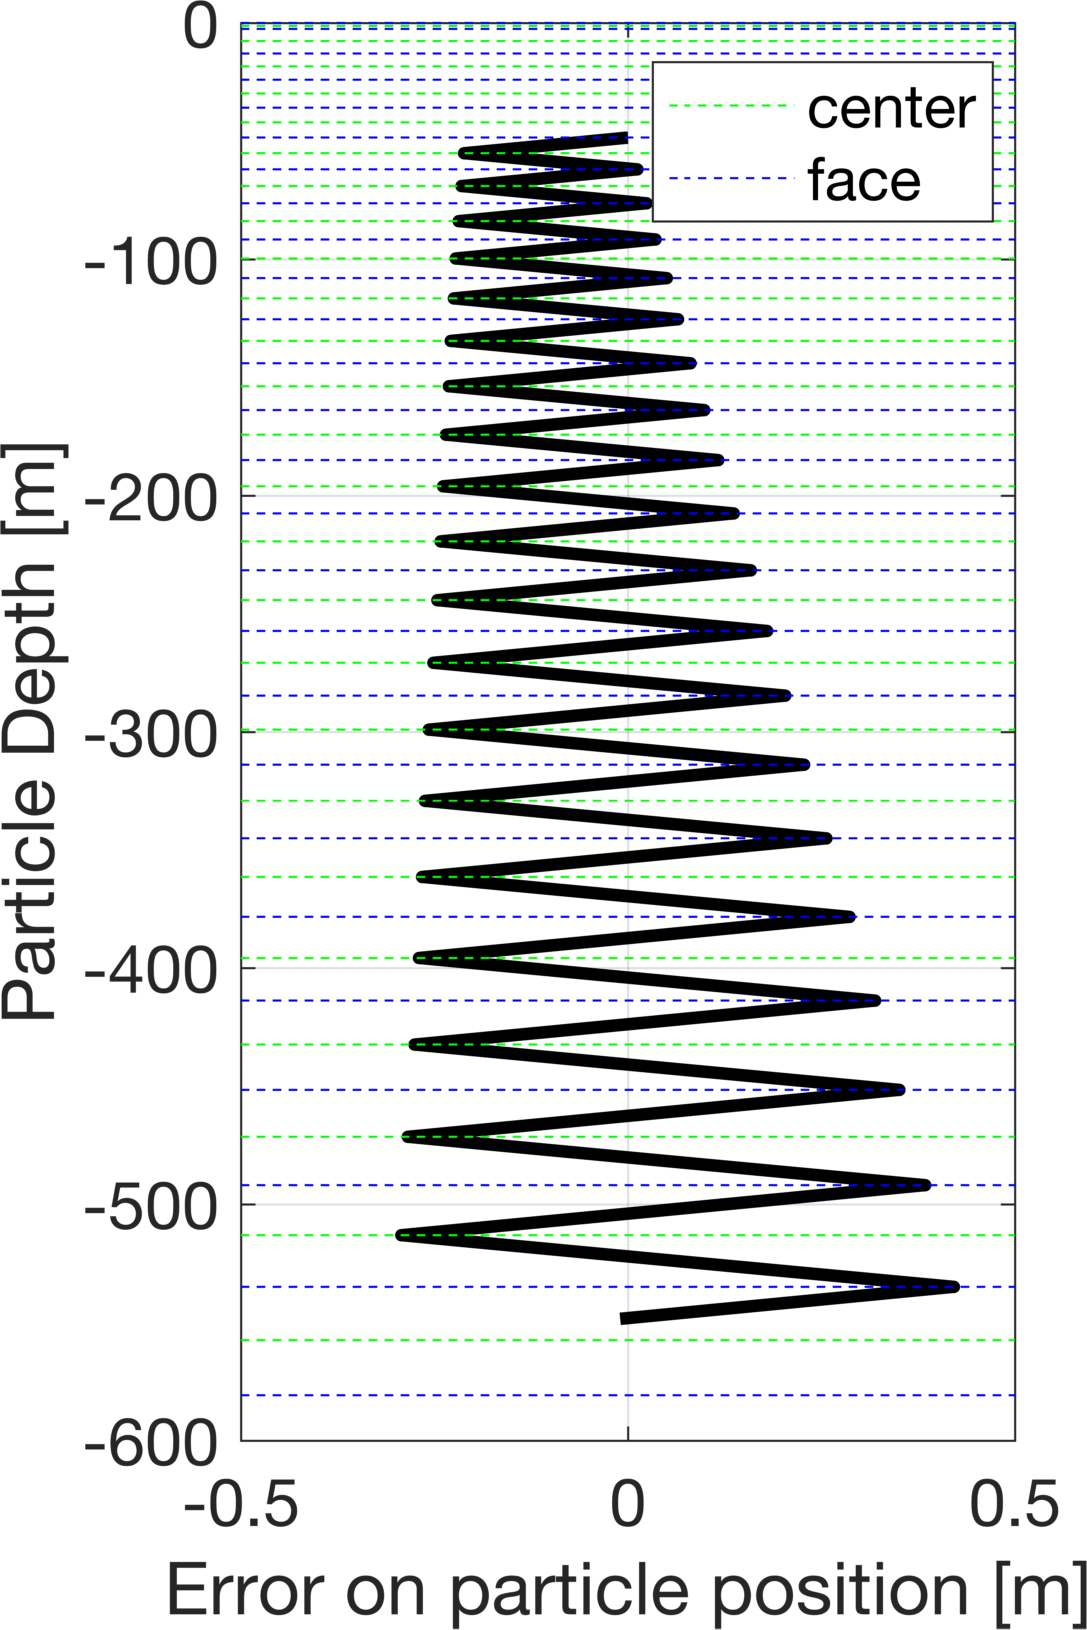
\includegraphics[width = .35\linewidth]{error.png}
	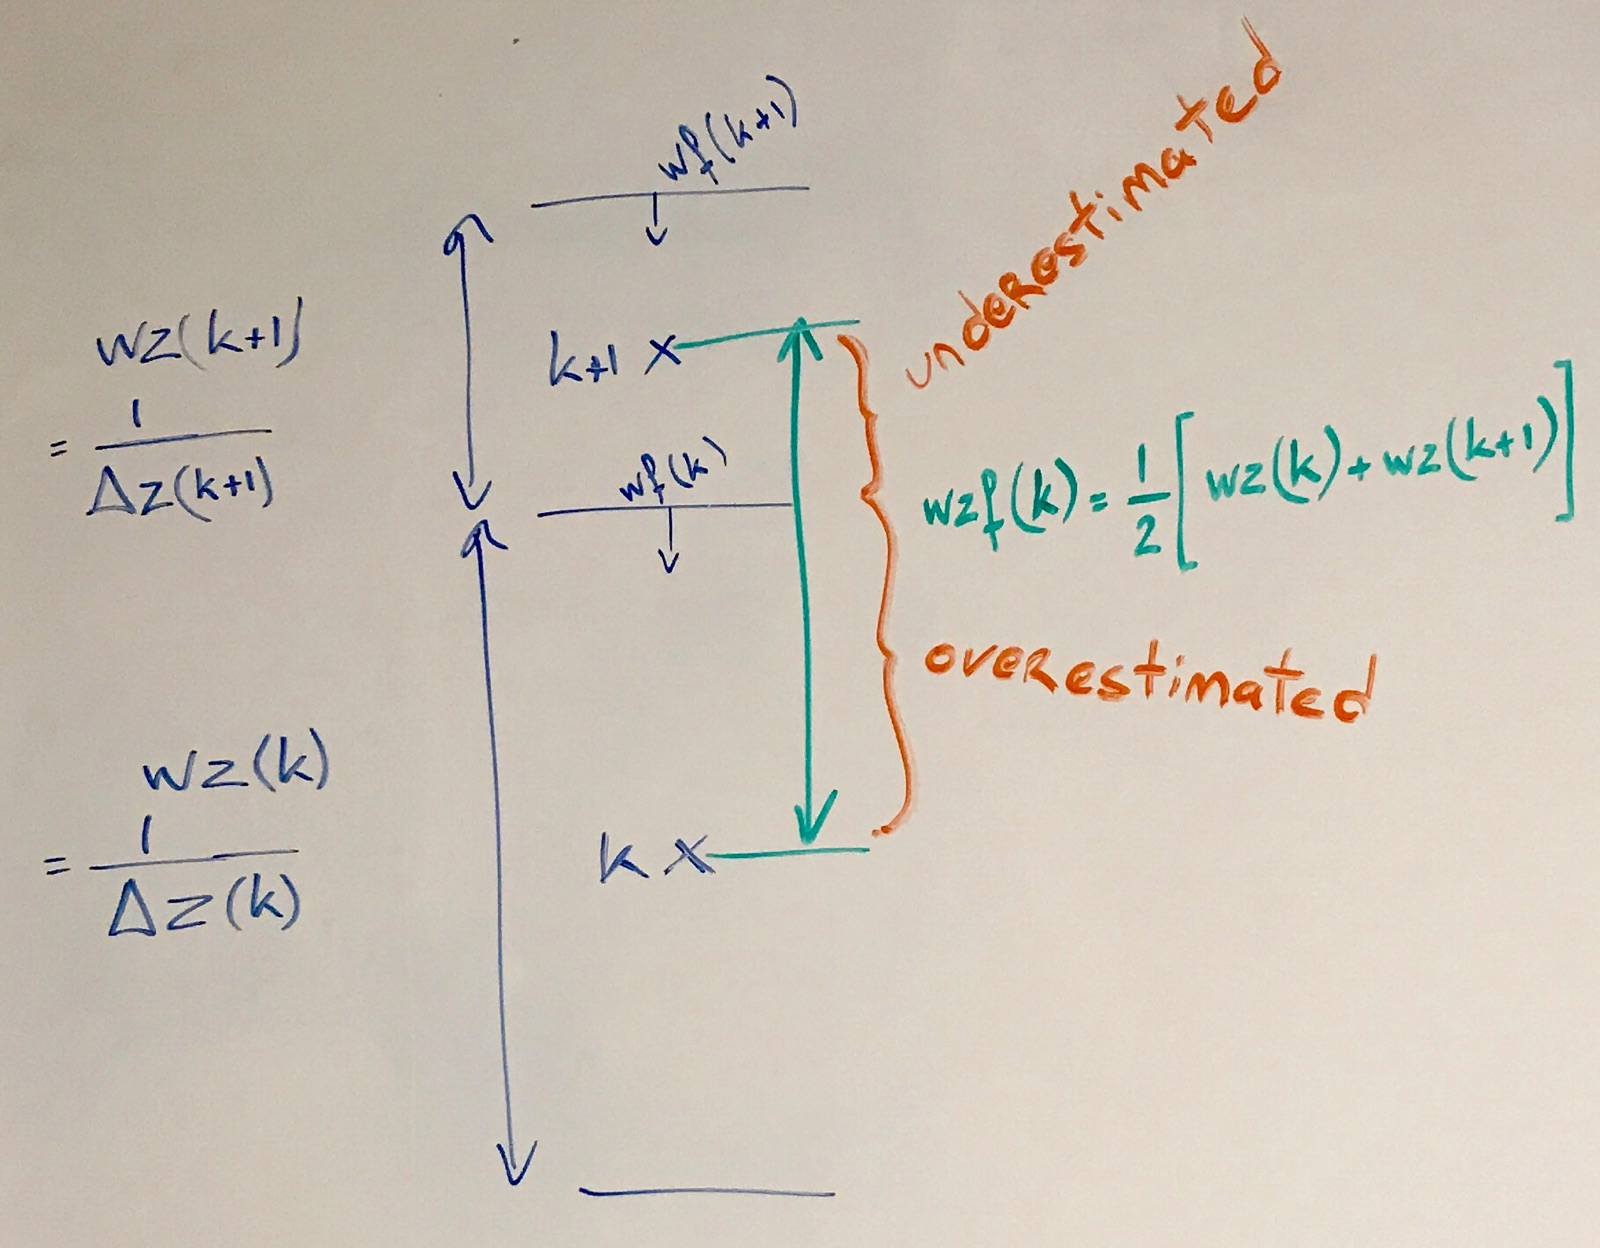
\includegraphics[width = .64\linewidth]{drawing.jpeg}
	\caption{\label{fig: model_depth_error} Error on particle vertical position due to the interpolation of $wzf$ onto the particle position. Error is maximum at model grid cell centers and at grid cell faces. Error grows with depth, as grid cells become thicker, and is independent of the sinking velocity. Right panel shows the important variables and highlights the limitations of the original method.}
\end{figure}

\subsection*{New approach}
Instead of relying on an interpolation of the discrete values of $wzf$, the continuous function that determines the depth of the k-levels (i.e., the vertical grid spacing), is used to exactly determine the value of $wzf$ at the particle's location. The function is defined in the routine \texttt{findz\_topmoves.f90}.

\begin{lstlisting}[language=fortran]
       zc(i,j,k)= (exp(pfac*xfac)-1.d0)*epm1inv*(D(i,j)+dztop) -dztop
\end{lstlisting}
which can be re-written in terms of set parameters as:
\marginnote{\raggedright \small \textbf{\underline{What is the constant C?}}\\The value of $C$ is irrelevant in this context, as the difference between two z-levels is the quantity we are ultimately interested in.}

\begin{equation} \label{eq: zc}
zc(i,j,k) = \left(\frac{D(i,j)+dztop}{e^{pfac}-1}\right)e^{pfac}e^{\frac{-pfac(k-0.5)}{NK-1}} + C 
\end{equation}
where $zc$ is the depth of the cell-center, $D(i,j)$ is the dimensionless depth of the 0-th face z (at cell centers in $x$ and $y$), $dztop$ is the dimensionless thickness of the uppermost cell, $pfac$ is the vertical stretching parameter used to define the sigma levels, $NK$ is the number of vertical levels, and $C$ is a constant.

The equation for the difference between two z-levels at k and k+1 (i.e., $\Delta z$) can thus be derived (Figure \ref{fig: Dz_derivation}):
\marginnote{\justifying \small \textbf{\underline{What about the horizontal?}}\\A slightly different equation than the one depicted in Figure \ref{fig: Dz_derivation} must be used if computing $wz$. While $wzf$ must be computed using the depth of the z-cell centers $zc$, $wz$ must be computed using the depths of the z-cell faces $zf$. this is achieved by using $k$ instead of $(k-0.5)$ in Equation \ref{eq: zc}.}

\begin{figure}[!h]
	\centering
	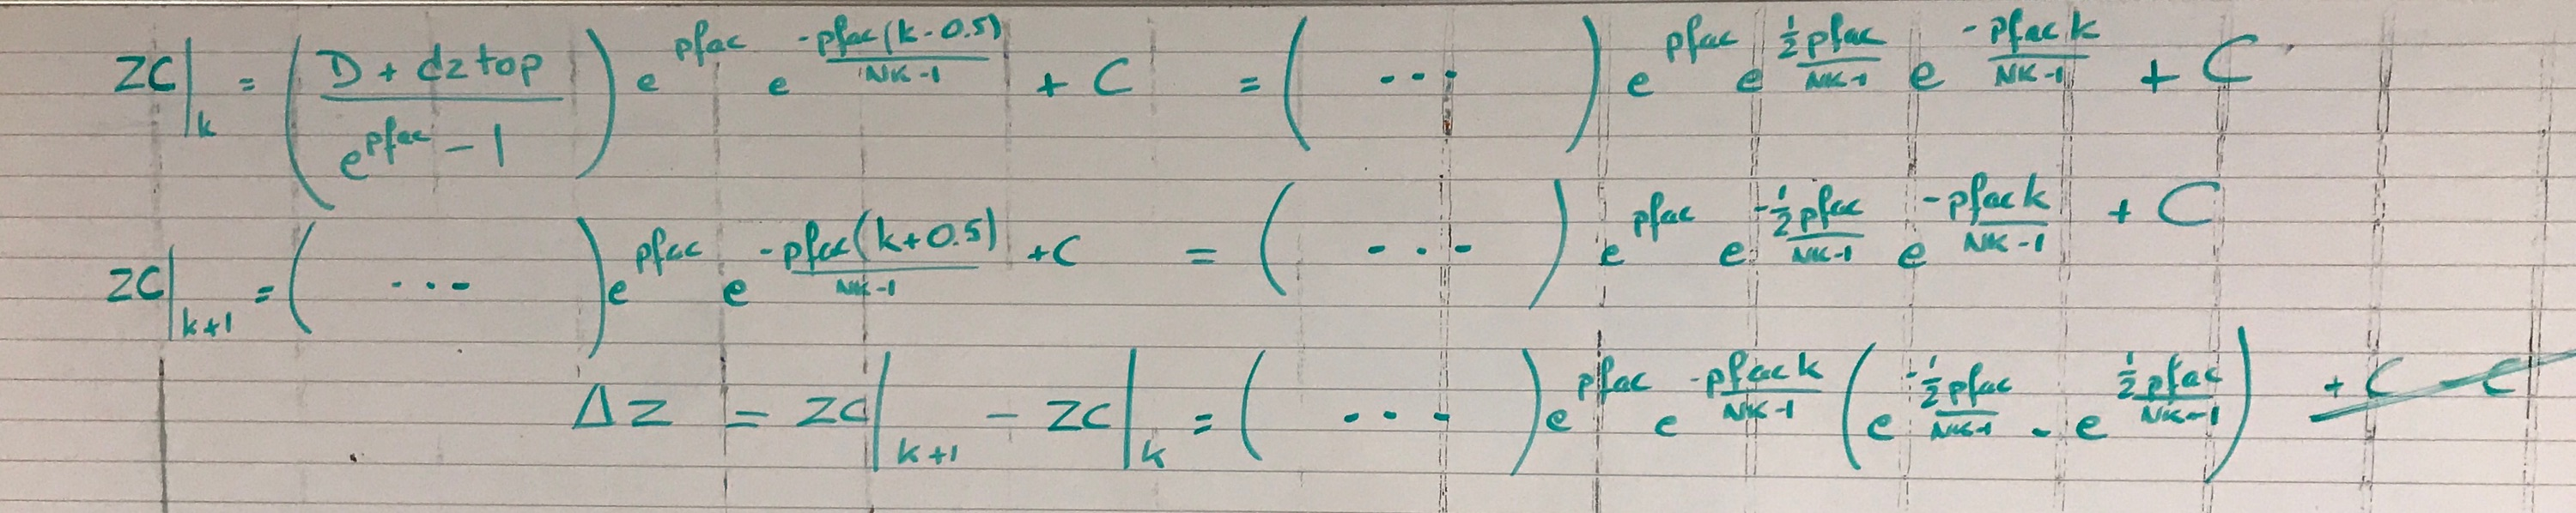
\includegraphics[width = \linewidth]{Dz_derivation.jpeg}
	\caption{\label{fig: Dz_derivation} Equations used to compute $\Delta z$ at k-faces in \texttt{particles.f90}}
\end{figure}

The variable $wzf$ can now be computed exactly at the particle's position by taking the inverse of $\Delta z$. Figure \ref{fig: no_model_error} shows the error (in meters, as well as in percentage of the particle's depth) on the particle vertical position after modifying the approach to compute $wzf$. The error grows linearly with depth, with a slope of 1.735 $\times$ 10$^{-4}$ m per meter (i.e., 17.35 cm at 1000 m deep).

\begin{figure}[!h]
	\centering
	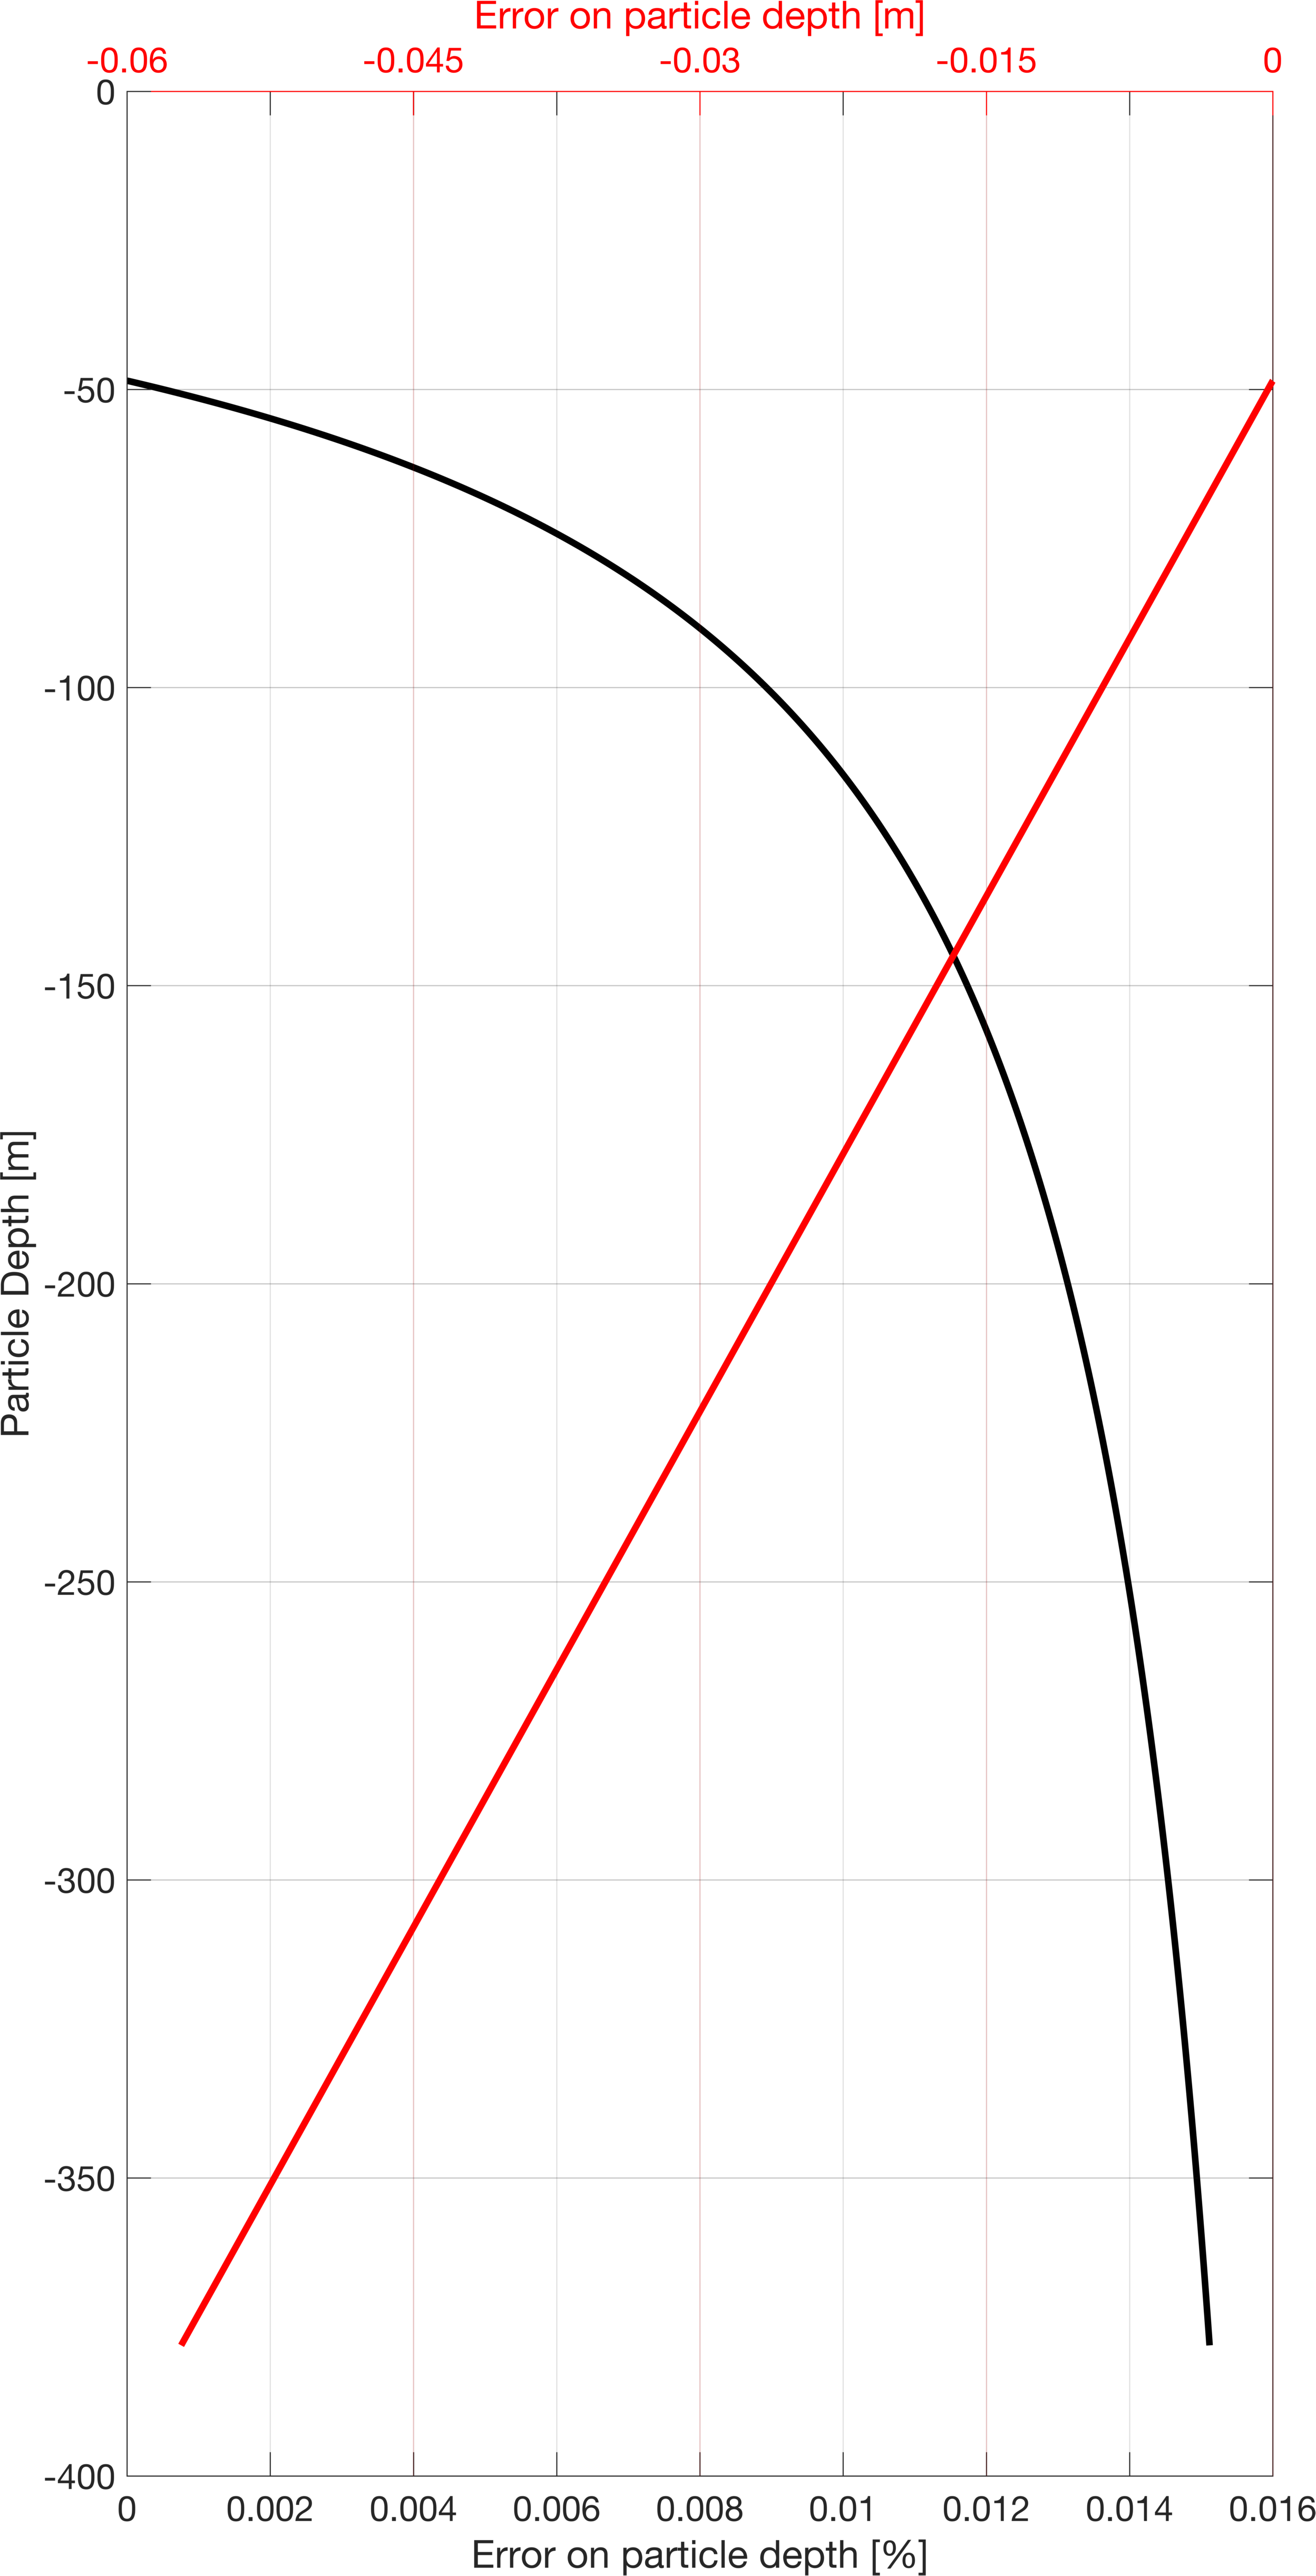
\includegraphics[width = .35\linewidth]{error_corrected.png}
	\caption{\label{fig: no_model_error} Error on particle vertical position after the approach used to compute $wzf$ was modified.}
\end{figure}
\end{document}